%ब
\chapter{Results and Discussions}
Performance of database systems is commonly measured in terms of the
\textit{Response time} and \textit{Throughput}(\todo{cite Demurjian, Berkely}).
Response time refers to the time  a database system takes to process an
operation and produce results to the end user . Measuring response time for a
database operation is similar to a black-box evaluation because it is measured 
without considering the internal functioning  of the database system. According
to (\todo{cite Demurjian}) such an evaluation is ideal for a complete database
system to measure its performance and to give the users details about its 
efficiency and speed in performing operations. In this thesis, response time and
throughput are the measures used to gauge the performance of Cassandra
while referential integrity validation is implemented using the \ac{API}.

Response time for each of the  operations that trigger such a validation from
all the solutions are measured during the experiments. This included the
time involved to access and retrieve metadata for the entities and also the time for
validating referential integrity by the \texttt{ValidationHandler}. The response
time of Cassandra when such validations are not in place is also measured and considered as a
baseline with which to analyse the solutions. Such a comparison  determines the degree of
change in speed of Cassandra when such overheads are introduced and gives 
users useful information about how each solution affects the performance of
the database system.

The second performance measure used is \textit{Throughput} which
is another classical and commonly used measure of database performance
(\todo{cite BerkleyDB}).
Throughput measures the number of operations processed by the database system in a unit of
time. Across all solutions in the experiments, the throughput for all the
operations triggering referential integrity validation  is measured
as operations per second.
A single operation stands for each time an entity is inserted, updated or
deleted. Note that only the operations that
introduce the referential integrity validation in Cassandra is measured and thus
\texttt{read} operations are not measured in terms of response time or
throughput.

It has to be noted that the operations are prone to  external factors like
network latency, bandwidth, network routing, network workload among others which
typically affect a network consisting of several machines and users. This is
because the Cassandra cluster used in the experiments is deployed over a
network that is used by many users concurrently thus exposing the operations to
such factors. Identifying such factors and analysing them is beyond the scope of
this thesis and the analysis is strictly in terms of how the metadata storage
and referential integrity validation affects Cassandra's performance.

 The results from the experiments were used to
analyse the performance of the four solutions with respect to  response
time and throughput and this is discussed in the following sections.
Section~\ref{sr:baseline} presents the results for the baseline experiment where 
% no referential validation checks are implemented
% and t
the operations performed on the entities are just as it would be performed in
Cassandra. Section~\ref{sr:insert} analyses the results of all the solutions
for the \texttt{insert} operation. Section~\ref{sr:update} presents the analysis
for the \texttt{update} operation for all the solutions. Section~\ref{sr:delete}
discusses the results of the solutions for the \texttt{delete} operation. 


\newcommand{\Width}{0.5\textwidth}
\newcommand{\TB}[1]{\textbf{#1}}

\section{Overview}


\todo{add to tables the unit (seconds, entities per second)}

\todo{Present tables and what they mean}

\todo{Explain why solution 4 is generally better except for update and delete
student}

\newcolumntype{B}{>{\columncolor{light-gray}}c} 
\begin{table}[h]
 \centering
\caption{Response time}\label{t:}
\begin{tabular}{ccBcccc}
\toprule
&&\textbf{Baseline} & \textbf{Solution1} & \textbf{Solution2} & \textbf{Solution3} & \textbf{Solution4}\\
\midrule
\multirow{3}{*}{\textbf{insert}} & \textbf{s} & 0.624 (0.138) & 0.714 (0.029) &
1.140 (0.057) & 3.444 (0.070) & \TB{0.686 (0.039)}\\
 & \textbf{c} & 0.630 (0.069) & 0.721 (0.027) & 1.181 (0.087) & 3.447 (0.096) &
 \TB{0.684 (0.030)}\\
 & \textbf{e} & 5.708 (0.310) & 16.883 (0.278) & 34.220 (1.399) & 55.359 (0.351)
 & \TB{15.340 (0.276)}\\
\midrule
\multirow{3}{*}{\textbf{update}} & \textbf{s} & 1.254 (0.051) & \TB{32.312
(1.207)} & 67.080 (1.386) & 113.579 (1.495) & 48.000 (1.537)\\
 & \textbf{c} & 1.376 (0.099) & \TB{7.559 (0.297)} & 10.885 (0.384) & 19.279
 (0.252) & 7.580 (0.288)\\
 & \textbf{e} & 7.237 (0.425) & 18.228 (0.276) & 35.673 (1.402) & 56.762 (0.420)
 & \TB{16.694 (0.386)}\\
\midrule
\multirow{3}{*}{\textbf{delete}} & \textbf{s} & 0.592 (0.022) & \TB{10.798
(0.409)} & 18.952 (0.600) & 42.544 (0.619) & 35.919 (0.576)\\
 & \textbf{c} & 0.627 (0.023) & 3.602 (0.092) & 4.828 (0.118) & 6.745 (0.120) &
 \TB{3.324 (0.079)}\\
 & \textbf{e} & 5.847 (0.294) & 5.904 (0.359) & 12.282 (0.650) & 35.070 (0.472)
 & \TB{5.879 (0.240)}\\
\bottomrule
\end{tabular}
\end{table}



\begin{table}[h]
 \centering
\caption{Response time ratio}\label{t:}
\begin{tabular}{ccBcccc}
\toprule
&&\textbf{Baseline} & \textbf{Solution1} & \textbf{Solution2} & \textbf{Solution3} & \textbf{Solution4}\\
\midrule
\multirow{3}{*}{\textbf{insert}} & \textbf{s} & 0.62 & 1.14 & 1.83 & 5.52 &
\TB{1.10}\\
 & \textbf{c} & 0.63 & 1.14 & 1.87 & 5.47 & \TB{1.09}\\
 & \textbf{e} & 5.71 & 2.96 & 6.00 & 9.70 & \TB{2.69}\\
\midrule
\multirow{3}{*}{\textbf{update}} & \textbf{s} & 1.25 & \TB{25.76} & 53.48 &
90.55 & 38.27\\
 & \textbf{c} & 1.38 & \TB{5.49} & 7.91 & 14.01 & 5.51\\
 & \textbf{e} & 7.24 & 2.52 & 4.93 & 7.84 & \TB{2.31}\\
\midrule
\multirow{3}{*}{\textbf{delete}} & \textbf{s} & 0.59 & \TB{18.24} & 32.02 &
71.88 & 60.68\\
 & \textbf{c} & 0.63 & 5.74 & 7.70 & 10.76 & \TB{5.30}\\
 & \textbf{e} & 5.85 & 1.01 & 2.10 & 6.00 & \TB{1.01}\\
\bottomrule
\end{tabular}
\end{table}






\begin{table}[h]
 \centering
\caption{Throughput}\label{t:}
\begin{tabular}{ccBcccc}
\toprule
&&\textbf{Baseline} & \textbf{Solution1} & \textbf{Solution2} & \textbf{Solution3} & \textbf{Solution4}\\
\midrule
\multirow{3}{*}{\textbf{insert}} & \textbf{s} & 1634 (157) & 1403 (56) & 880
(41) & 290 (6) & \TB{1463 (71)}\\
 & \textbf{c} & 1598 (108) & 1389 (52) & 851 (61) & 290 (7) & \TB{1465 (62)}\\
 & \textbf{e} & 1756 (70) & 592 (9) & 293 (12) & 181 (1) & \TB{652 (11)}\\
\midrule
\multirow{3}{*}{\textbf{update}} & \textbf{s} & 798 (30) & \TB{31 (1)} & 15 (0)
& 9 (0) & 21 (1)\\
 & \textbf{c} & 730 (43) & \TB{132 (5)} & 92 (3) & 52 (1) & 132 (5)\\
 & \textbf{e} & 1385 (62) & 549 (8) & 281 (11) & 176 (1) & \TB{599 (13)}\\
\midrule
\multirow{3}{*}{\textbf{delete}} & \textbf{s} & 1692 (61) & \TB{93 (3)} & 53 (2)
& 24 (0) & 28 (0)\\
 & \textbf{c} & 1597 (57) & 278 (7) & 207 (5) & 148 (3) & \TB{301 (7)}\\
 & \textbf{e} & 1714 (80) & 1700 (95) & 817 (45) & 285 (4) & \TB{1704 (64)}\\
\bottomrule
\end{tabular}
\end{table}



\begin{table}[h]
\newcommand{\B}[1]{\colorbox{light-gray}{#1}}
 \centering
\caption{Throughput inverse ratio}\label{t:}
\begin{tabular}{ccBcccc}
\toprule
&&\textbf{Baseline} & \textbf{Solution1} & \textbf{Solution2} & \textbf{Solution3} & \textbf{Solution4}\\
\midrule
\multirow{3}{*}{\textbf{insert}} & \textbf{s} & 1634 & 1.17 & 1.86 & 5.63 &
\TB{1.12}\\
 & \textbf{c} & 1598 & 1.15 & 1.88 & 5.51 & \TB{1.09}\\
 & \textbf{e} & 1756 & 2.96 & 6.00 & 9.72 & \TB{2.69}\\
\midrule
\multirow{3}{*}{\textbf{update}} & \textbf{s} & 798 & \TB{25.77} & 53.54 & 90.67
& 38.29\\
 & \textbf{c} & 730 & \TB{5.51} & 7.93 & 14.06 & 5.52\\
 & \textbf{e} & 1385 & 2.52 & 4.93 & 7.86 & \TB{2.31}\\
\midrule
\multirow{3}{*}{\textbf{delete}} & \textbf{s} & 1692 & \TB{18.24} & 32.03 &
71.96 & 60.75\\
 & \textbf{c} & 1597 & 5.75 & 7.71 & 10.77 & \TB{5.31}\\
 & \textbf{e} & 1714 & 1.01 & 2.10 & 6.01 & \TB{1.01}\\
\bottomrule
\end{tabular}
\end{table}





\newpage
\section{Insert}

	\subsection{Student}
		\begin{figure}[H]
			\subfigure[Response time]
			{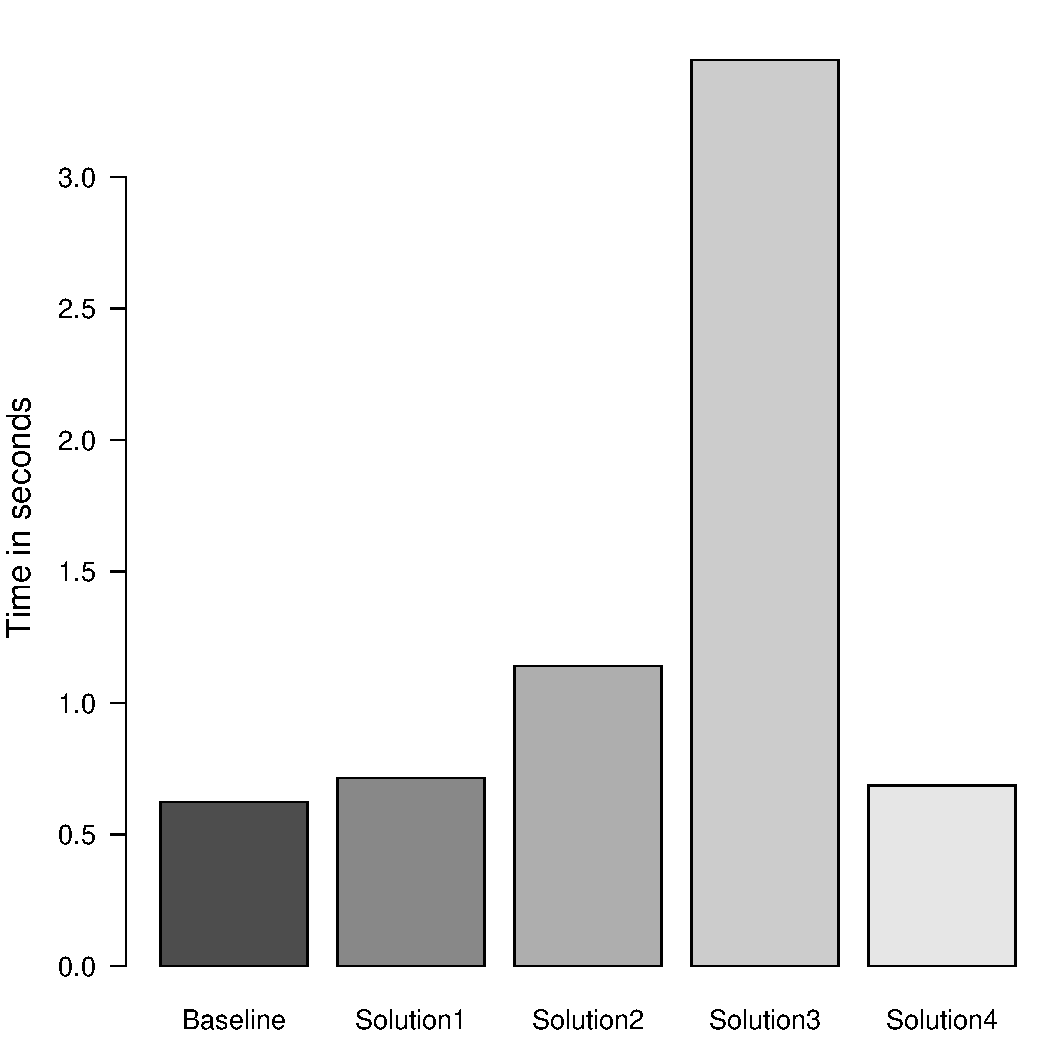
\includegraphics[width=\Width]{figure/result/barplot-insert_user-rt.pdf}}
			\subfigure[Throughput]
			{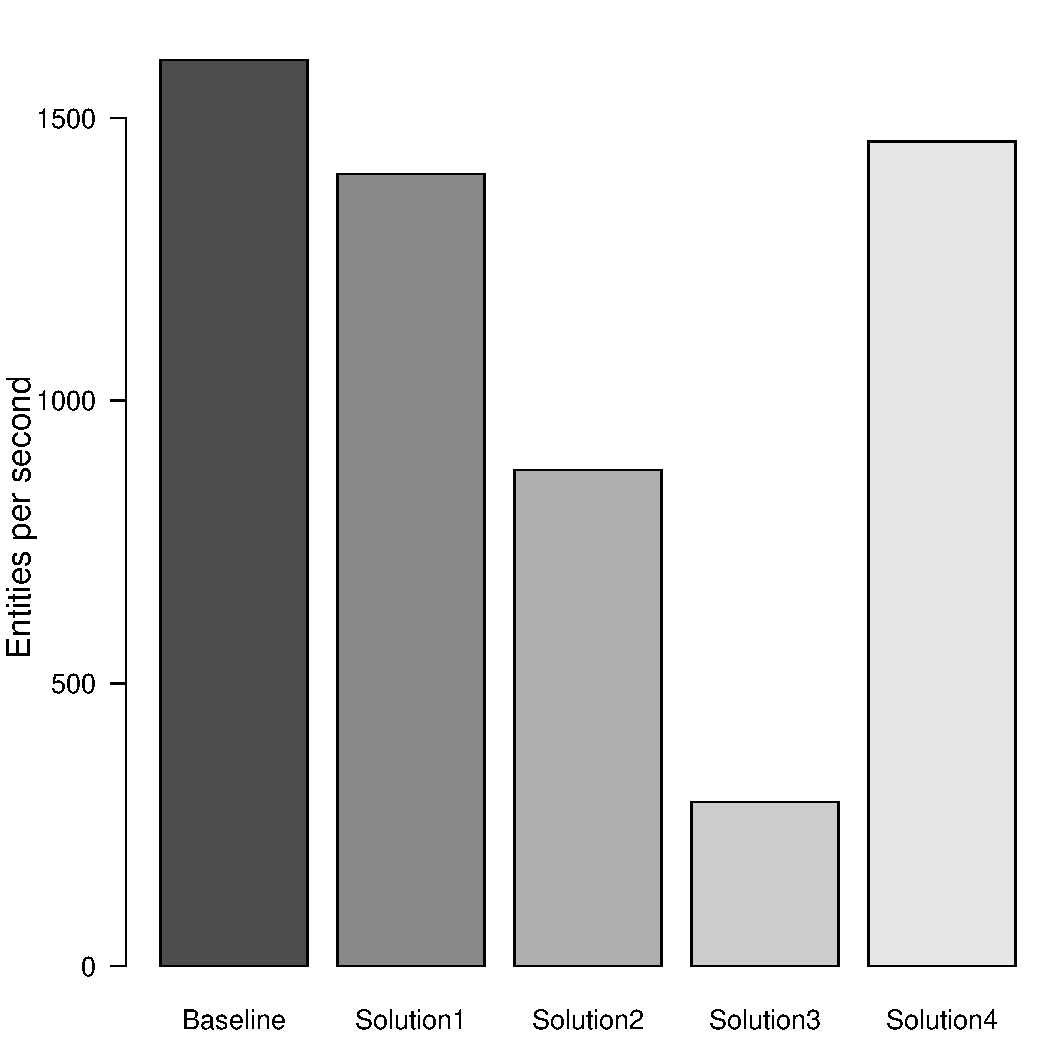
\includegraphics[width=\Width]{figure/result/barplot-insert_user-tp.pdf}}
			\caption{Performance inserting students}\label{f:rd:insert-user}
		\end{figure}
\newpage
	\subsection{Course}
		\begin{figure}[H]
			\subfigure[Response time]
			{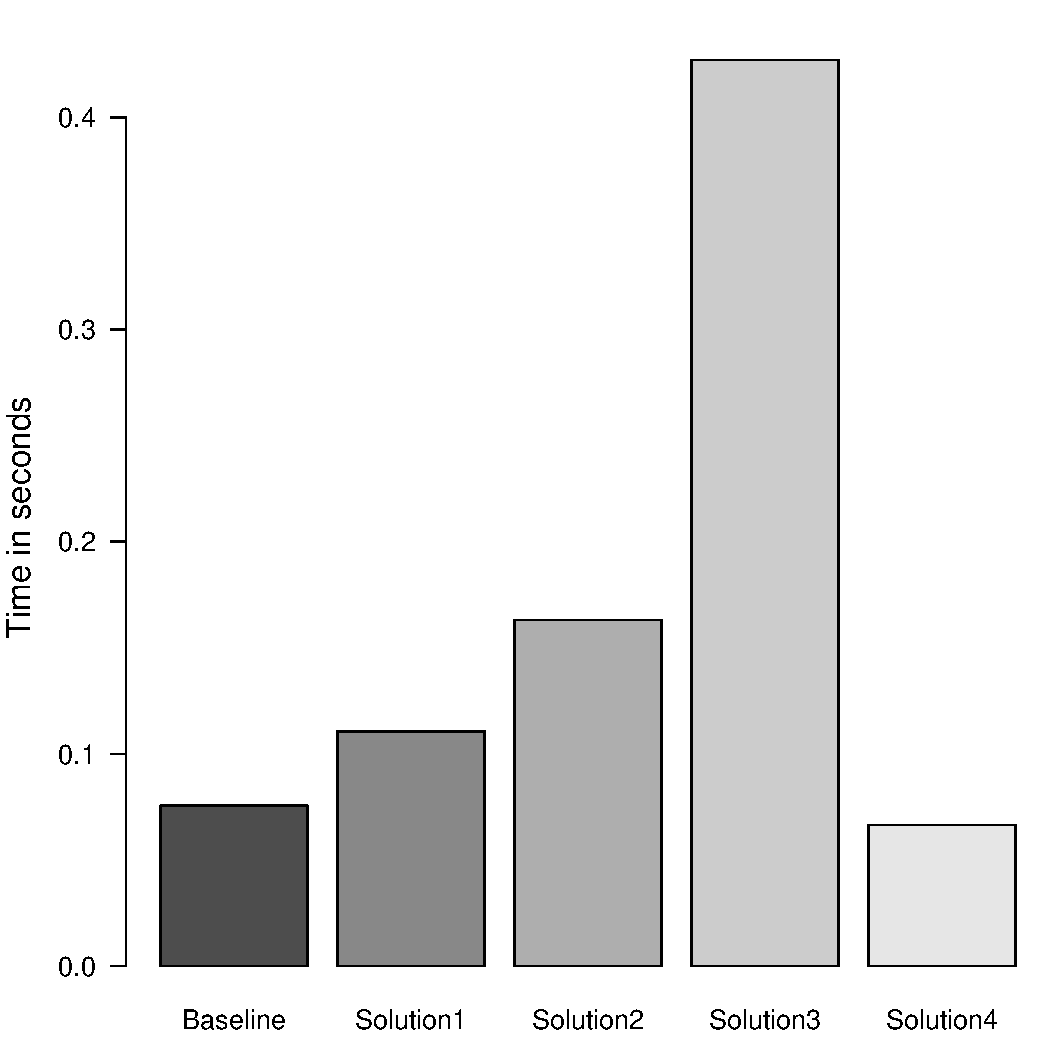
\includegraphics[width=\Width]{figure/result/barplot-insert_course-rt.pdf}}
			\subfigure[Throughput]
			{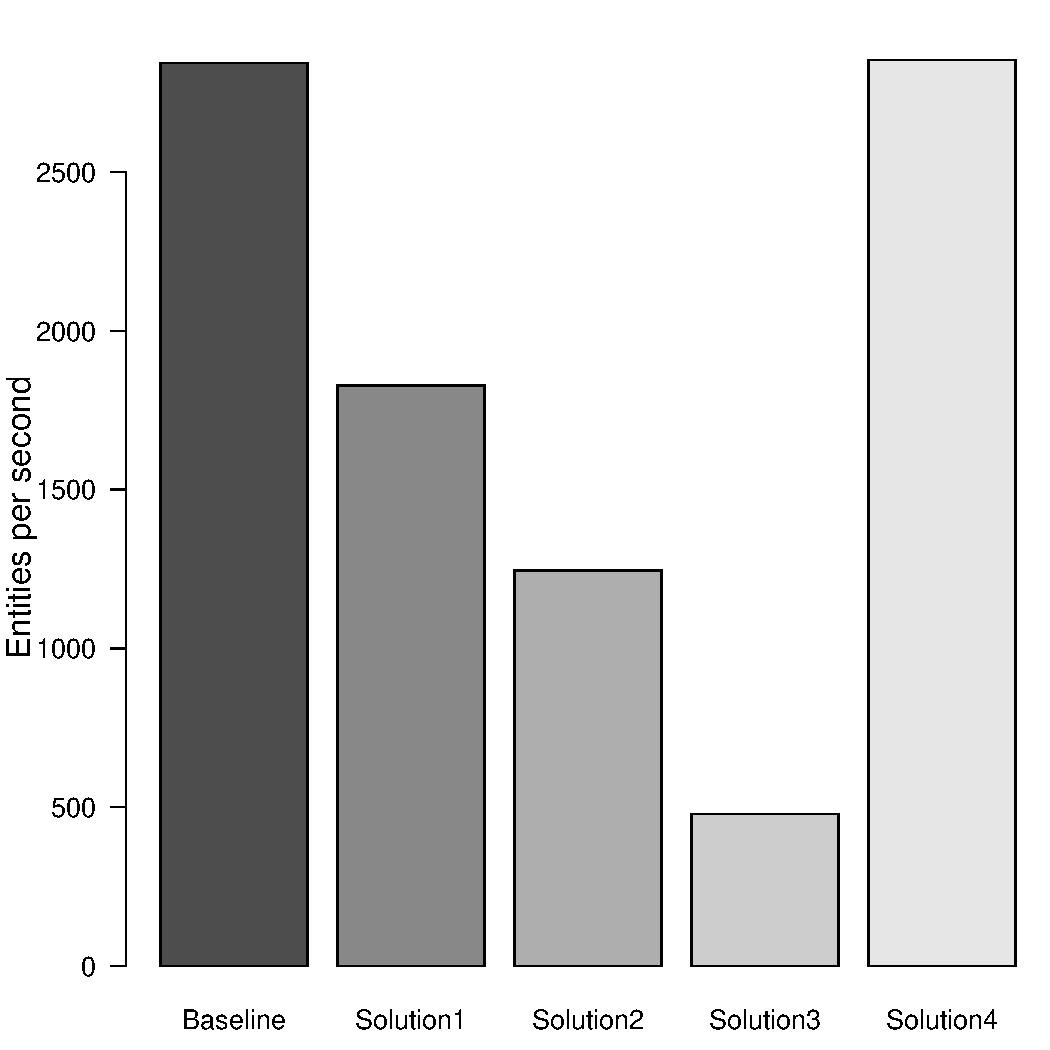
\includegraphics[width=\Width]{figure/result/barplot-insert_course-tp.pdf}}
			\caption{Performance inserting courses}\label{f:rd:insert-course}
		\end{figure}	
\newpage	
	\subsection{Enrolment}
		\begin{figure}[H]
			\subfigure[Response time]
			{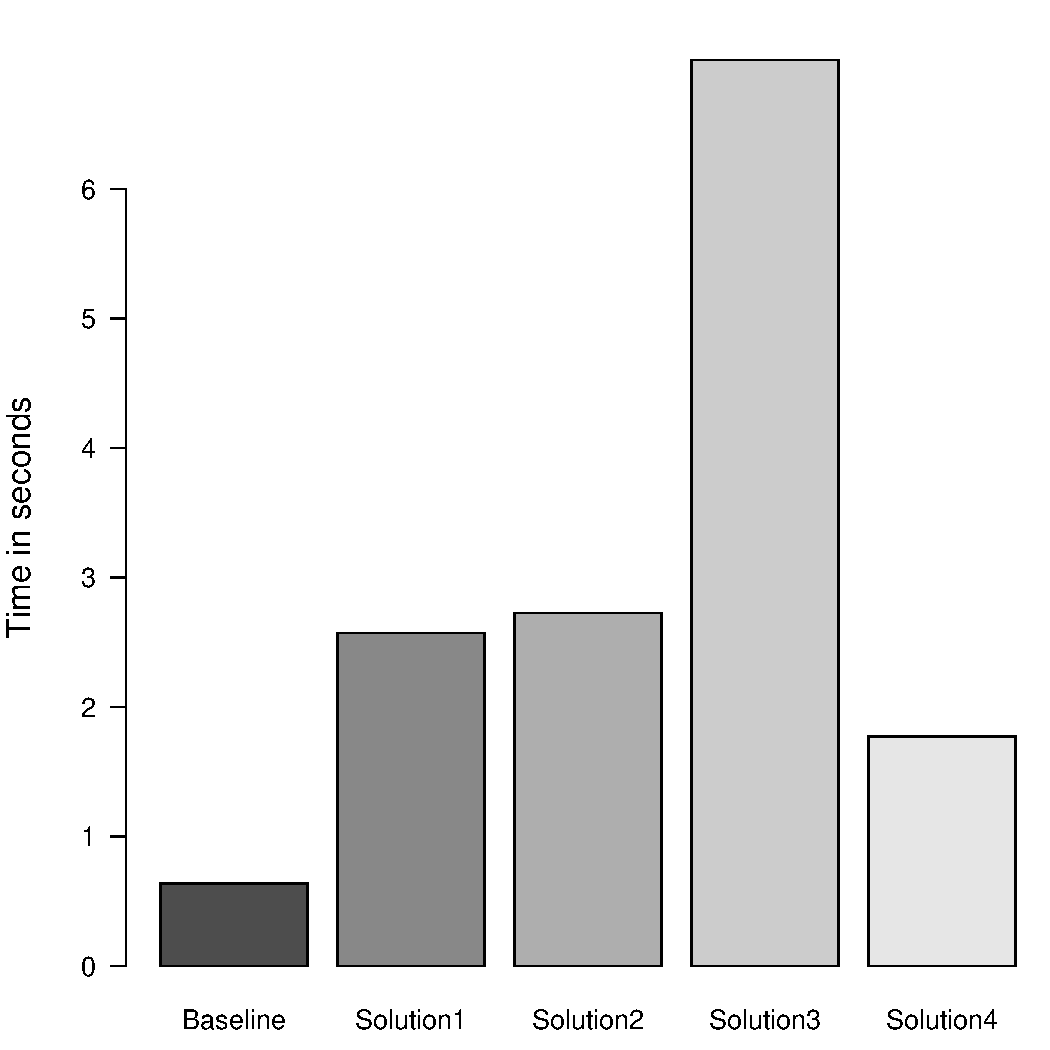
\includegraphics[width=\Width]{figure/result/barplot-insert_enrolment-rt.pdf}}
			\subfigure[Throughput]
			{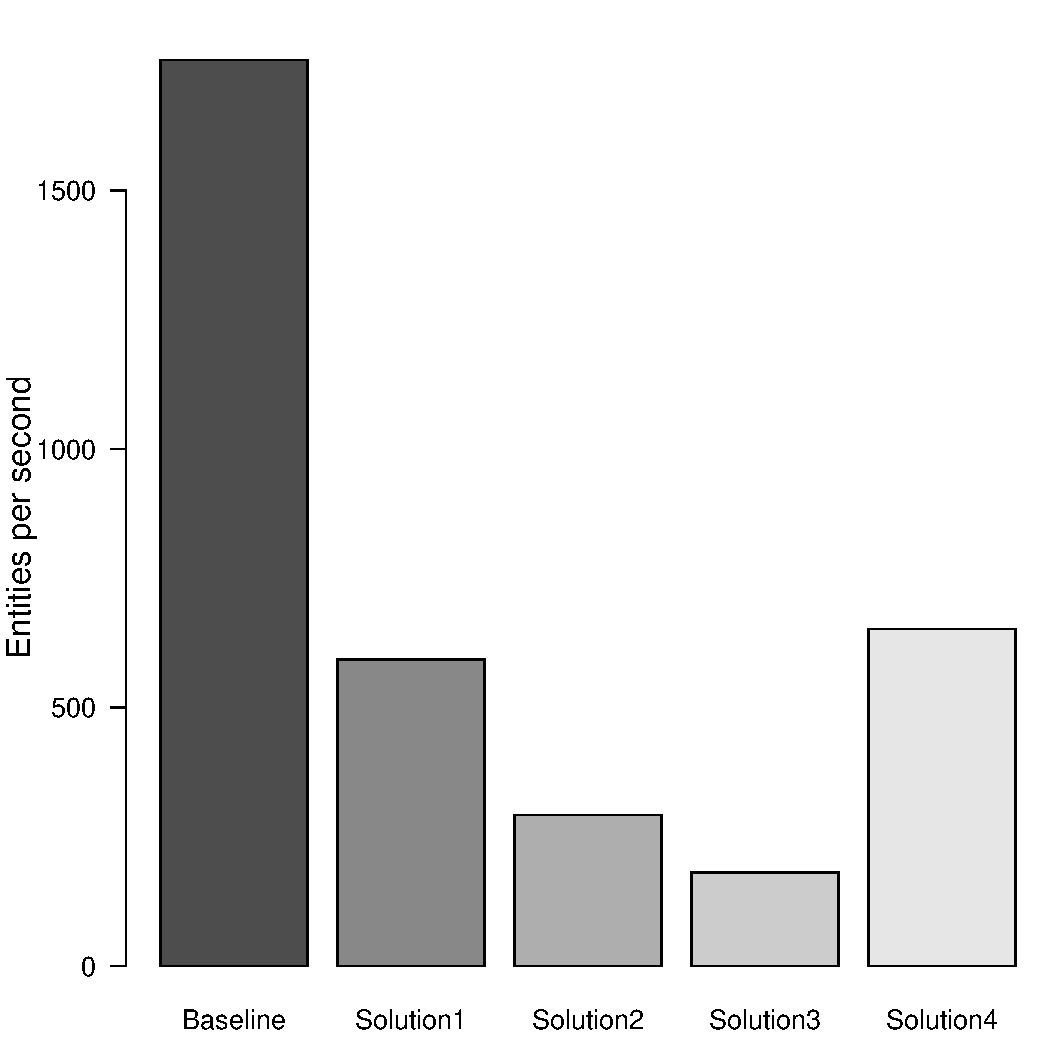
\includegraphics[width=\Width]{figure/result/barplot-insert_enrolment-tp.pdf}}
			\caption{Performance inserting enrolments}\label{f:rd:insert-enrolment}
		\end{figure}
		
\clearpage
\newpage
\section{Update}

	\subsection{Student}
		\begin{figure}[H]
			\subfigure[Response time]
			{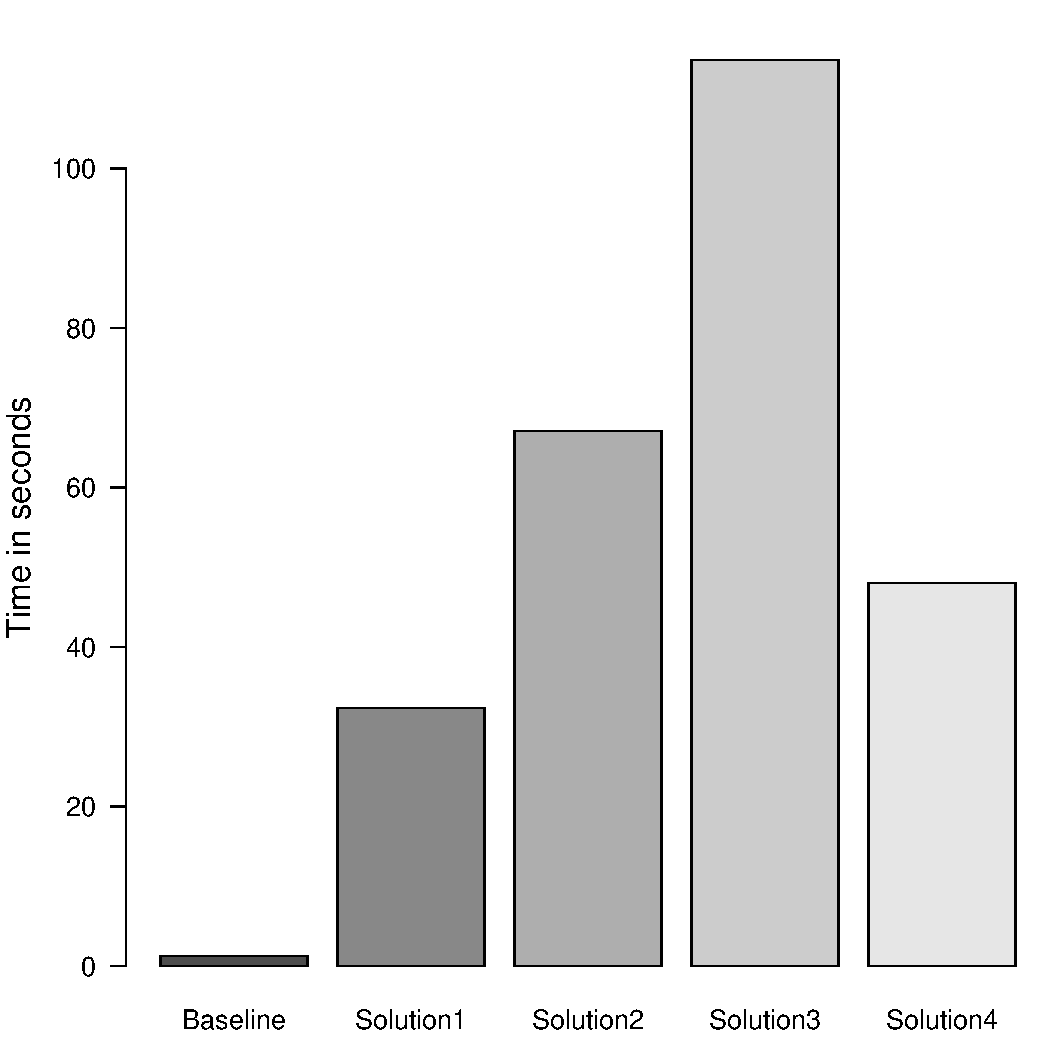
\includegraphics[width=\Width]{figure/result/barplot-update_user-rt.pdf}}
			\subfigure[Throughput]
			{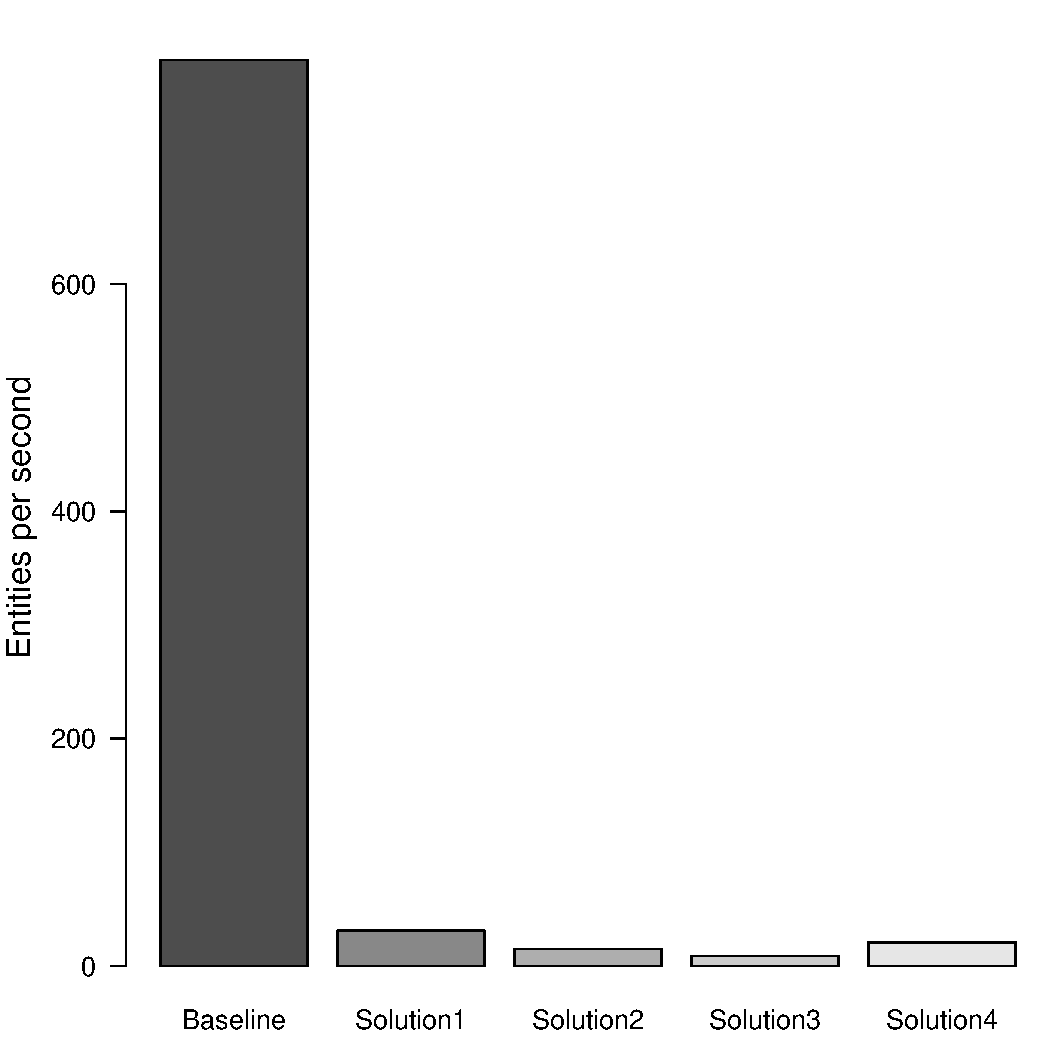
\includegraphics[width=\Width]{figure/result/barplot-update_user-tp.pdf}}
			\caption{Performance updating students}\label{f:rd:update-user}
		\end{figure}
\newpage	
	\subsection{Course}
		\begin{figure}[H]
			\subfigure[Response time]
			{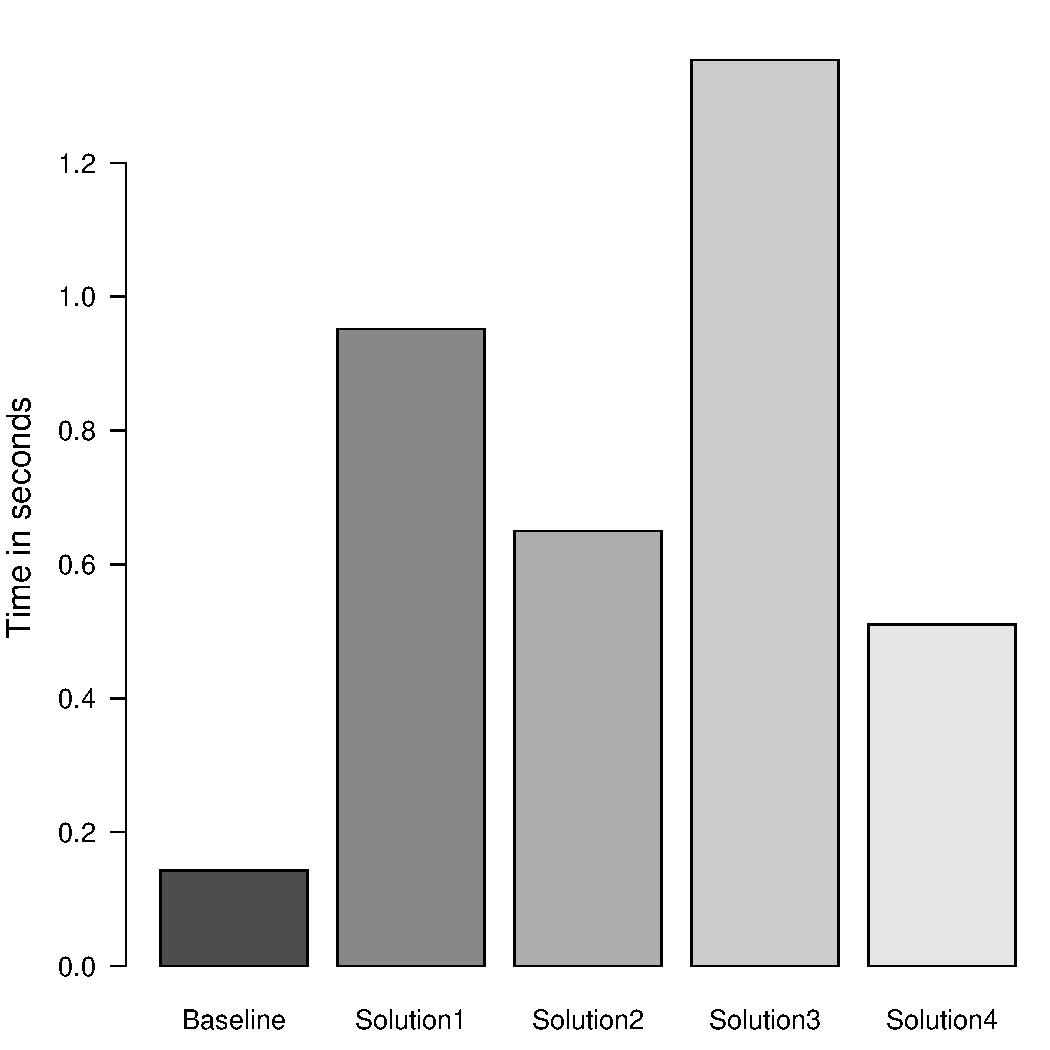
\includegraphics[width=\Width]{figure/result/barplot-update_course-rt.pdf}}
			\subfigure[Throughput]
			{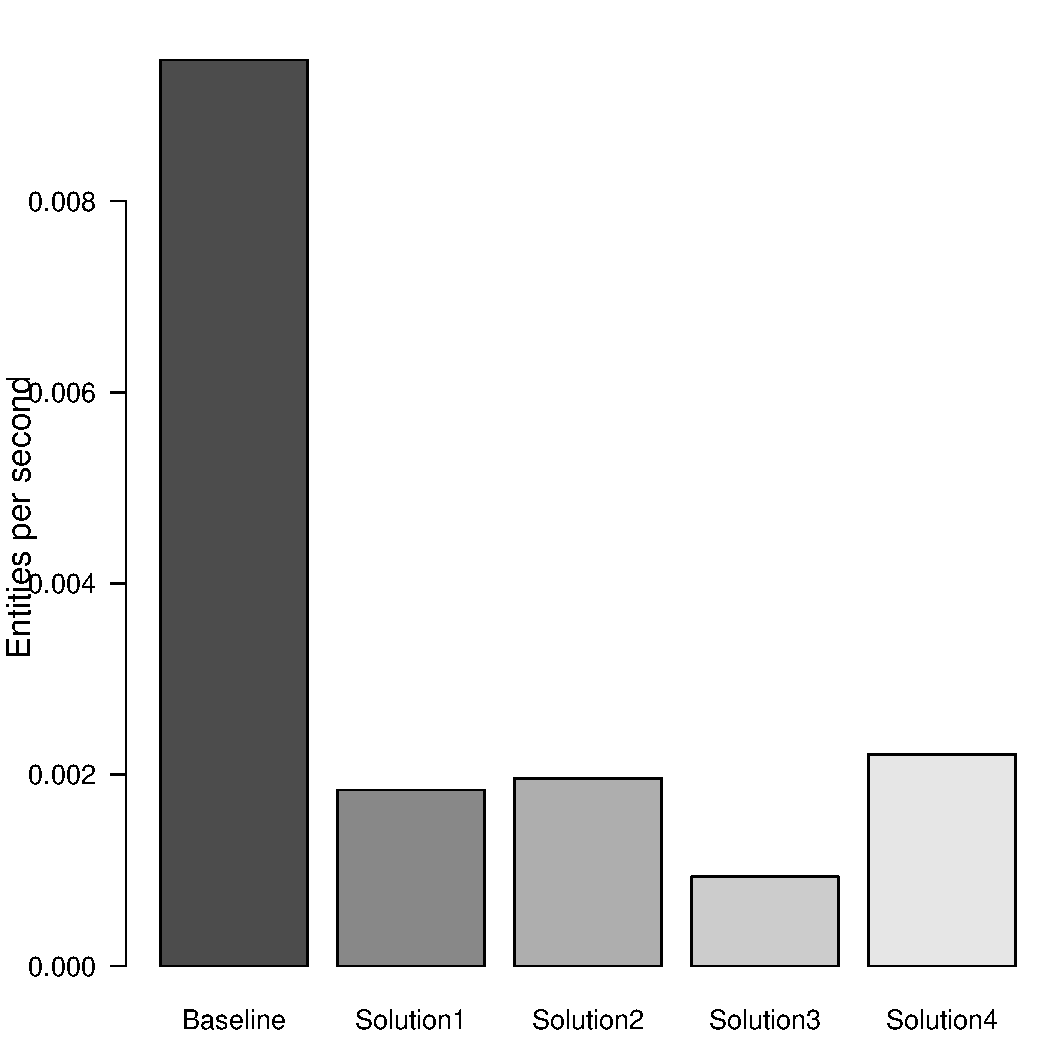
\includegraphics[width=\Width]{figure/result/barplot-update_course-tp.pdf}}
			\caption{Performance updating courses}\label{f:rd:update-course}
		\end{figure}	
\newpage	
	\subsection{Enrolment}
		\begin{figure}[H]
			\subfigure[Response time]
			{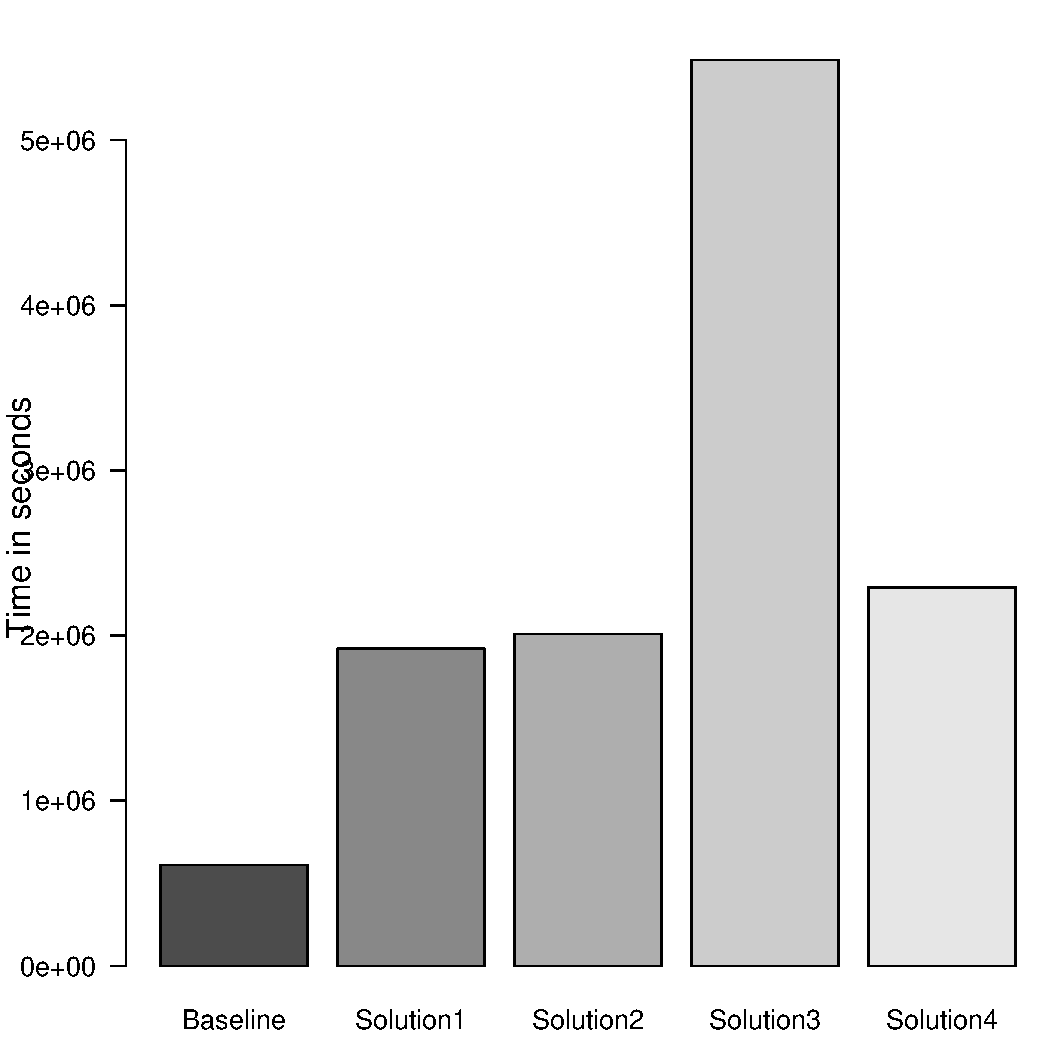
\includegraphics[width=\Width]{figure/result/barplot-update_enrolment-rt.pdf}}
			\subfigure[Throughput]
			{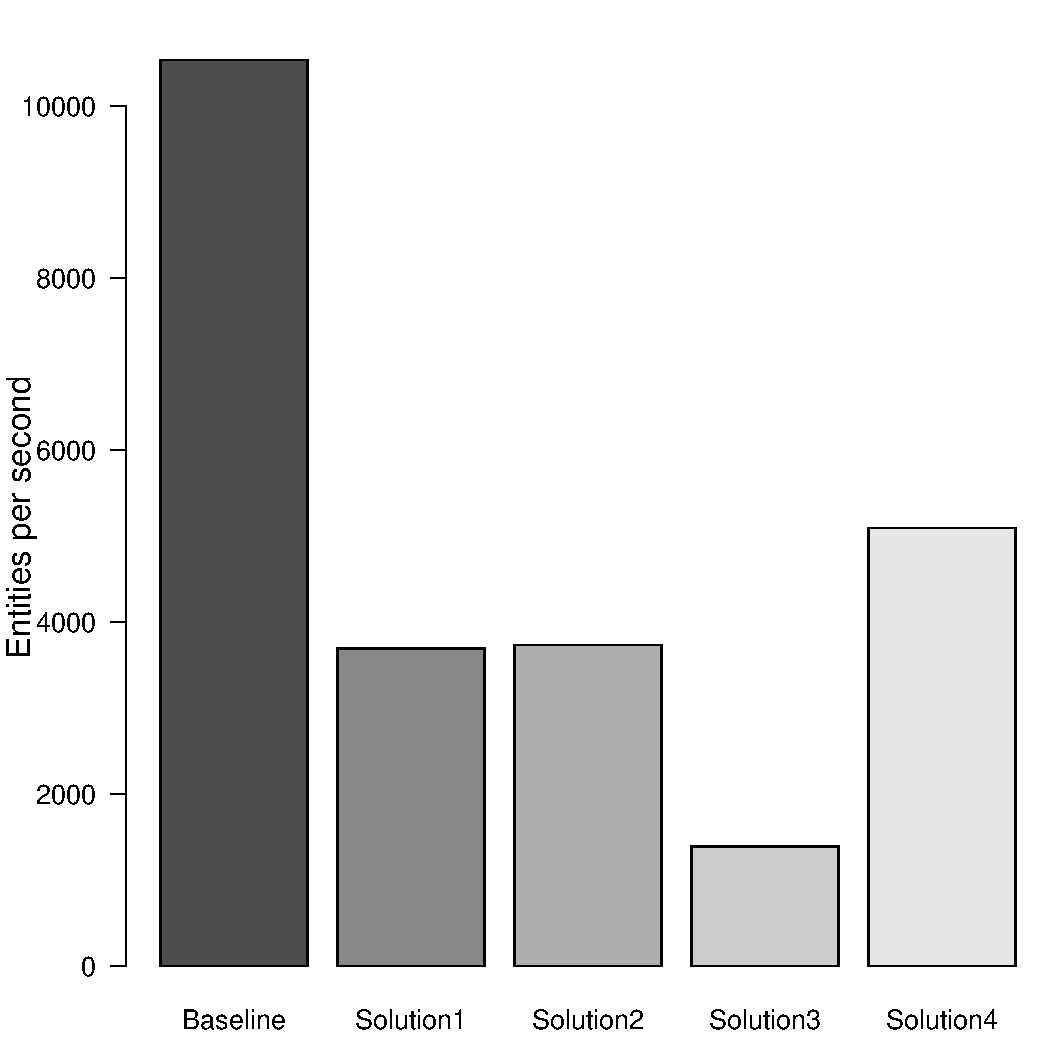
\includegraphics[width=\Width]{figure/result/barplot-update_enrolment-tp.pdf}}
			\caption{Performance updating enrolments}\label{f:rd:update-enrolment}
		\end{figure}
\clearpage
\newpage
\section{Delete} 

	\subsection{Student}
		\begin{figure}[H]
			\subfigure[Response time]
			{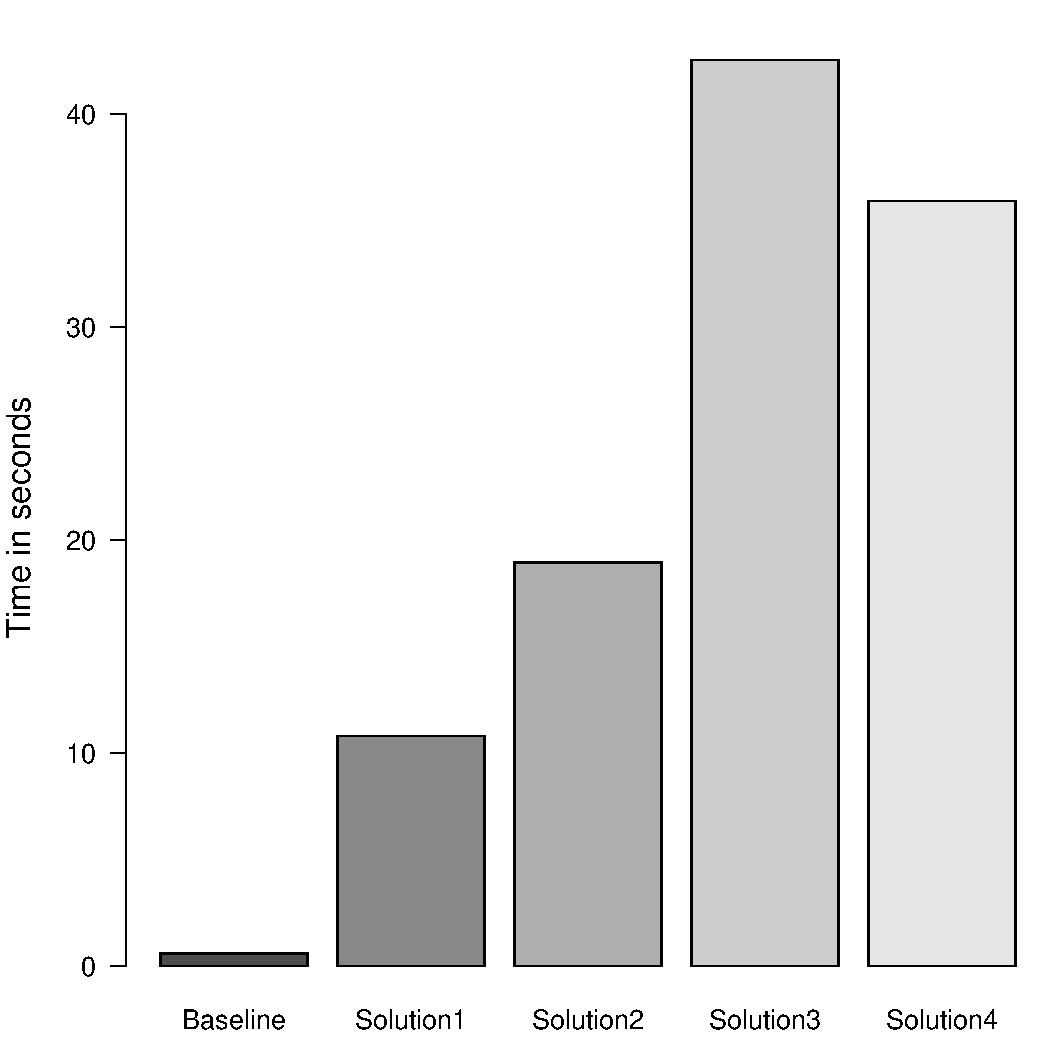
\includegraphics[width=\Width]{figure/result/barplot-delete_user-rt.pdf}}
			\subfigure[Throughput]
			{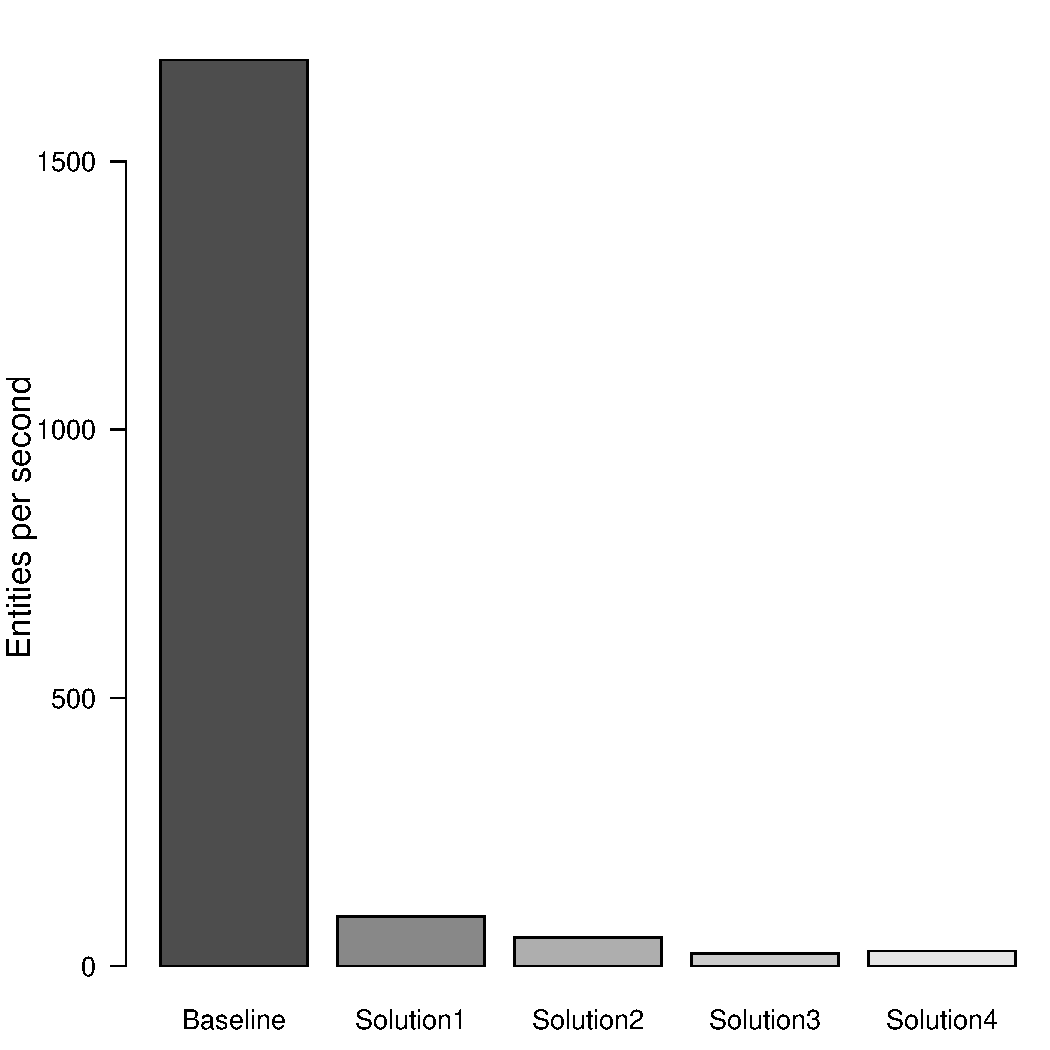
\includegraphics[width=\Width]{figure/result/barplot-delete_user-tp.pdf}}
			\caption{Performance deleting students}\label{f:rd:delete-user}
		\end{figure} 
\newpage	  
	\subsection{Course}
		\begin{figure}[H]
			\subfigure[Response time]
			{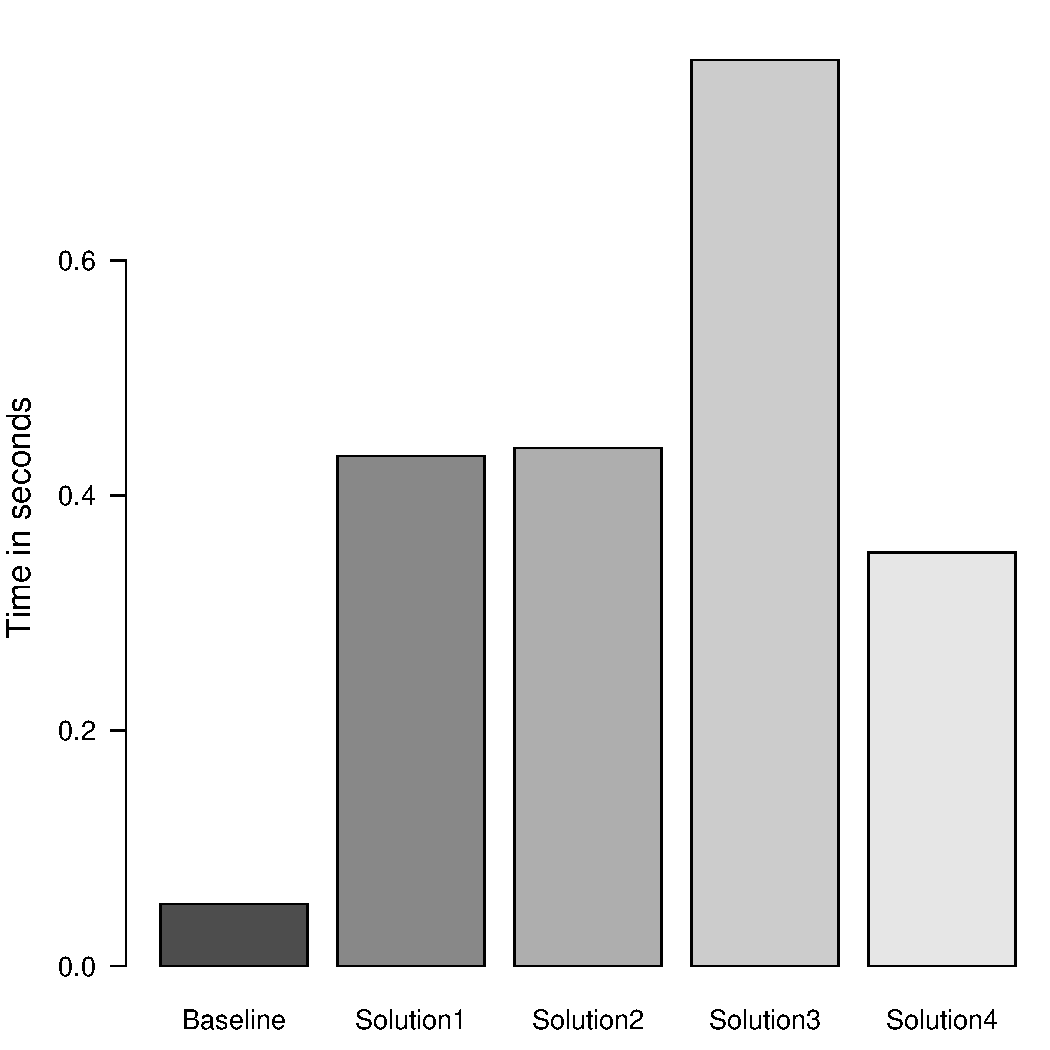
\includegraphics[width=\Width]{figure/result/barplot-delete_course-rt.pdf}}
			\subfigure[Throughput]
			{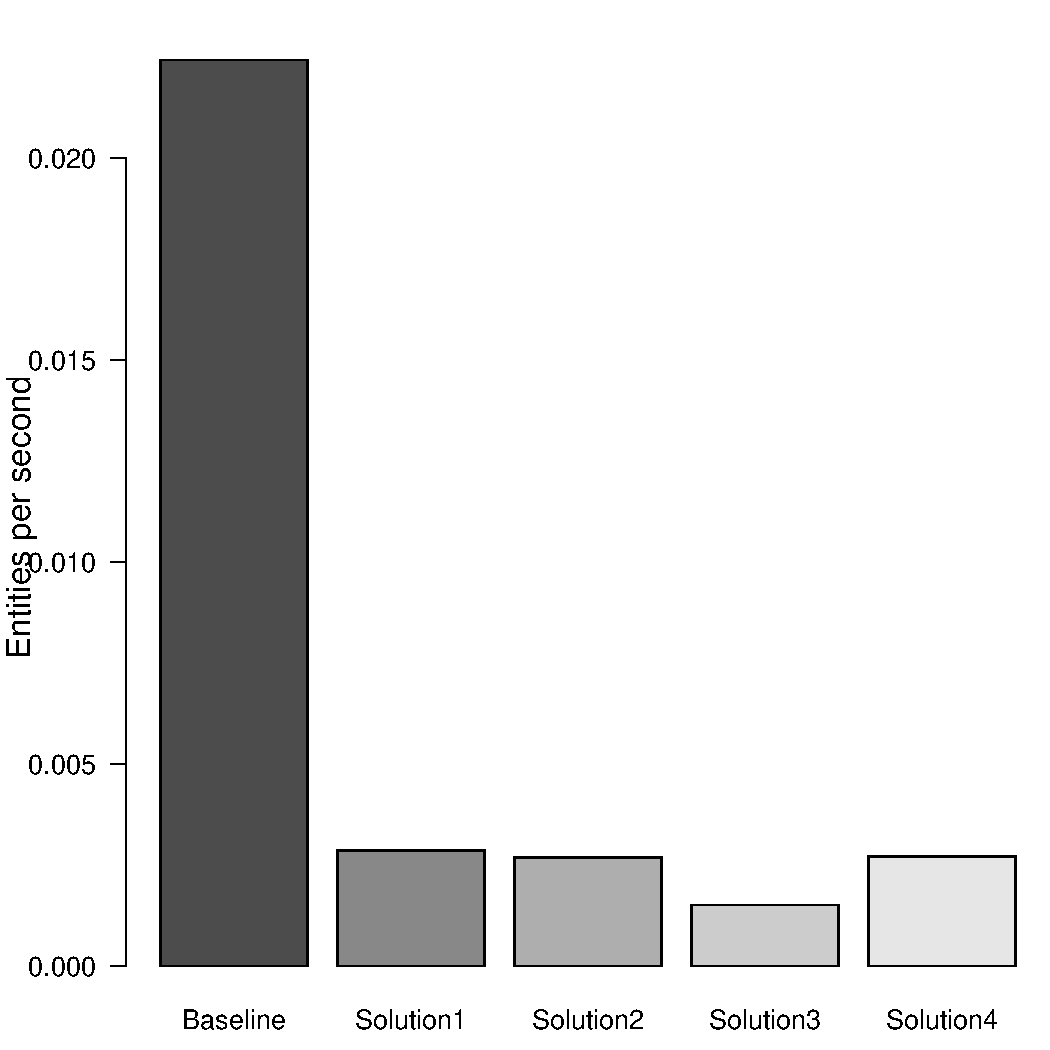
\includegraphics[width=\Width]{figure/result/barplot-delete_course-tp.pdf}}
			\caption{Performance deleting courses}\label{f:rd:delete-course}
		\end{figure}	
\newpage	 
	\subsection{Enrolment}
		\begin{figure}[H]
			\subfigure[Response time]
			{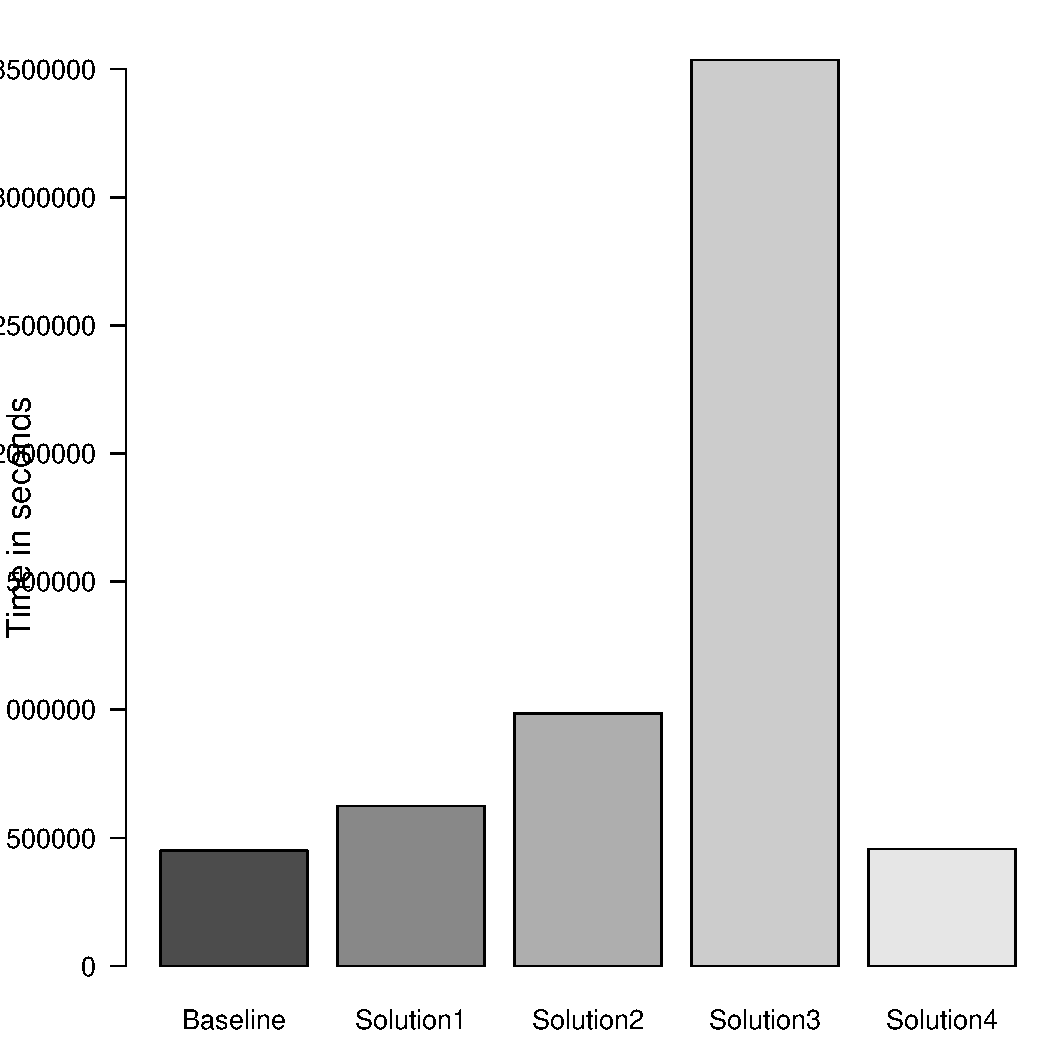
\includegraphics[width=\Width]{figure/result/barplot-delete_enrolment-rt.pdf}}
			\subfigure[Throughput]
			{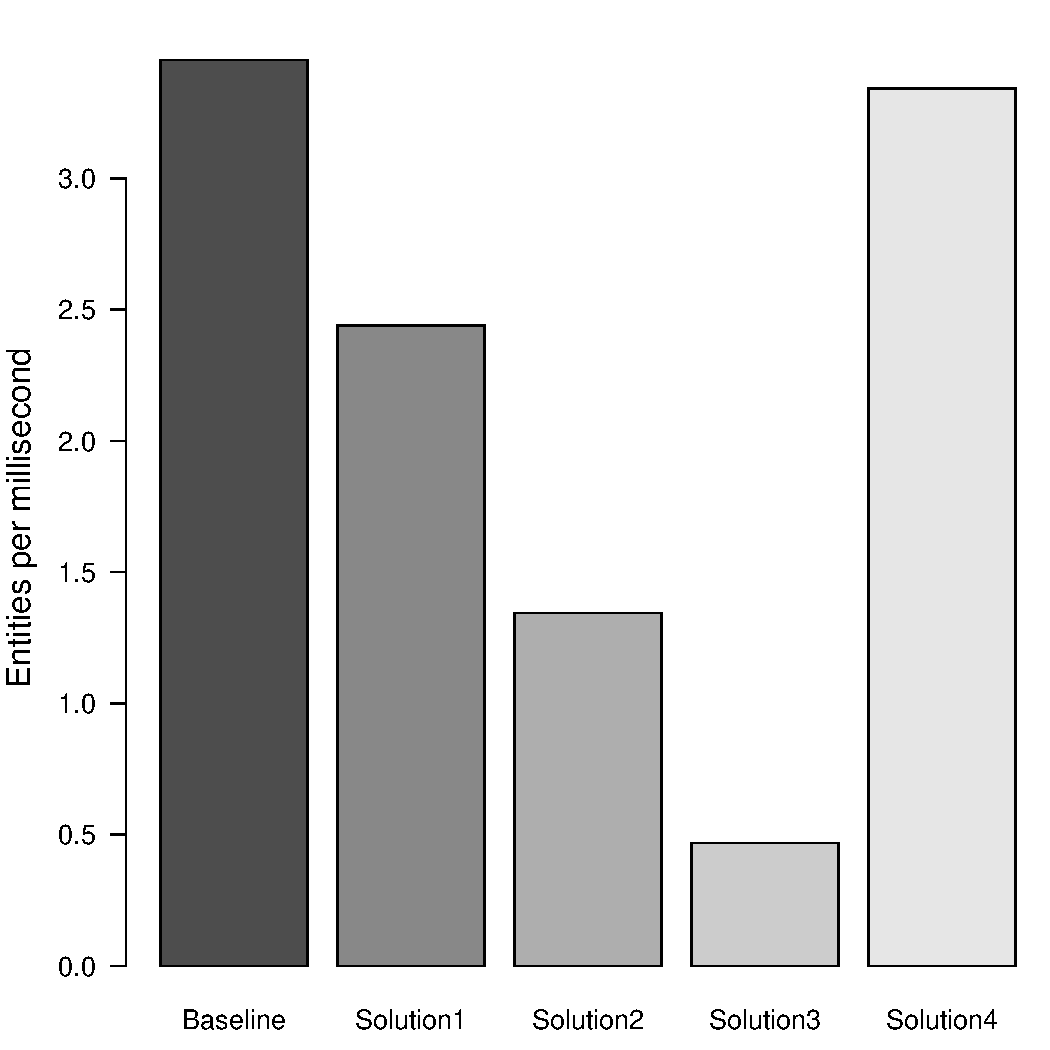
\includegraphics[width=\Width]{figure/result/barplot-delete_enrolment-tp.pdf}}
			\caption{Performance deleting enrolments}\label{f:rd:delete-enrolment}
		\end{figure}
		


	